\subsection{Life forms on Earth}

\initial{I}t is easy to forget the many shapes and styles life on our little planet takes. On a stroll along the seaside, you will walk past lifeforms so strange and different from you that when given deeper thought, they seem positively alien.
Consider the grass, which consumes sunlight to live and grow. Consider the life of the oyster, buried under the sand of the shoreline you walk past.
Consider the life of the seaweed, drifting at the surface, and how bizarre that existence seems when compared to your own.
We get used to it, since we see it all the time, but to give it thought and time to study can give a profound impression of the incredulity of life on Earth.

So, what kind of lifeforms exist on Earth?
Is it just one long list of different species, or are there ways to divide it on a more fundamental basis?
The second option is fortunately the right one.
When comparing life on a molecular level it can be divided into three primary groups (or domains): bacteria, archaebacterial and eukaryotes \cite{Eukaryotes}.
Bacteria and archaebacterial go under the collective term prokaryotes.
The difference between eukaryotes and prokaryotes is considered the most important distinction among living organisms \cite{Procaryotes}. 

\begin{center}
	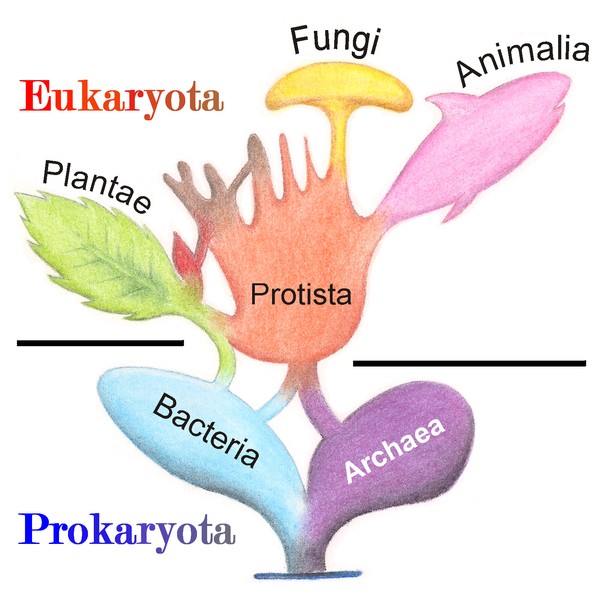
\includegraphics[width=0.45\textwidth]{Tree_of_living_organisms.jpg}
\end{center}

Prokaryotes are single-celled organisms living in clusters or colonies while eukaryotes can be both unicellular and multicellular.
Prokaryotes reproduce asexually meaning it clones itself, which we humans can't do quite yet, while most eukaryotes reproduce by mixing the parents genome \cite{ProcaEuka}. 

An easy way to consider this is that prokaryotes are like bacteria (very small and 'simple' life forms) and eukaryotes is the things that are more familiar to us, like plants, mushrooms, animals as well as you and me.
While complexity separates us, we all come from the same origins, which in and of itself is an astounding thought.

The theory is that the common universal ancestor of all life was a prokaryotic cell and that the eukaryotes were created by prokaryotes fusing \cite{ProcaEuka}.
This is analogous to us, as human beings. You think of yourself as just \textit {yourself}, don't you? The being behind the eyes, looking out, observing, thinking, interacting.
It's \textit{just you}.
'Just you', as complex as you are with your ability to laugh, love and create, is a living form consisting of trillions of other lifeforms, dancing together in a complicated dance every second of every day of your life.
All the cells in your body, all the external bacteria such as the flora in your gut that helps you digest food, all the enzymes and neurons and proteins, all can be considered their own living entities.
They all work together to make you \textit{you}, and all of this happens without your input.
The coordination between these lifeforms at the lowest level is natural and not planned - the cells in your hand don't meet with the cells in your lung at the pub and ask, 'hey, what do you do for a living?'
They aren't even aware of each others' existence.

\subsection{Virus, the odd one out}

\initial{T}he virus distinguishes itself from other biological beings on our planet by being the only kind which replicates within the cells of other lifeforms, and can do so within all other lifeforms on Earth\cite{koonin}. The virus is a tiny organism, and consists of DNA/RNA behind a protein suit of armor, that is removed when the virus enters a potential host cell. It then hijacks the host cells reproductive machinery and injects its own genes. The corrupted cells produce more virus, which can then infect nearby cells\cite{villareal}. The virus has a long history of debate as to whether its alive or not alive, and by modern definitions inhabit a grey area between the two, as it is unique in its way of survival and reproduction.